% Simplified Penrose Diagram - Schwarzschild Black Hole
% Replacing complex lightcones with simple orthogonal (x,t) arrows
\documentclass[border=3pt,tikz]{standalone}
\usepackage{tikz}
\usepackage{amsmath} % for \text
\usepackage{mathrsfs} % for \mathscr
\usepackage{xfp} % higher precision (16 digits?)
\usepackage[outline]{contour} % glow around text
\usetikzlibrary{decorations.markings,decorations.pathmorphing}
\usetikzlibrary{angles,quotes} % for pic (angle labels)
\usetikzlibrary{arrows.meta} % for arrow size
\contourlength{1.4pt}

\newcommand{\calI}{\mathscr{I}} %\mathcal
\tikzset{>=latex} % for LaTeX arrow head
\colorlet{myred}{red!80!black}
\colorlet{myblue}{blue!80!black}
\colorlet{mygreen}{green!80!black}
\colorlet{mydarkred}{red!50!black}
\colorlet{mydarkblue}{blue!50!black}
\colorlet{mylightblue}{mydarkblue!6}
\colorlet{mypurple}{blue!40!red!80!black}
\colorlet{mydarkpurple}{blue!40!red!50!black}
\colorlet{mylightpurple}{mydarkpurple!80!red!6}
\colorlet{myorange}{orange!40!yellow!95!black}

\tikzstyle{world line}=[myblue!60,line width=0.4]
\tikzstyle{world line t}=[mypurple!60,line width=0.4]
\tikzstyle{particle}=[mygreen,line width=0.5]
\tikzstyle{photon}=[-{Latex[length=4,width=3]},myorange,line width=0.4,decorate,
                    decoration={snake,amplitude=0.9,segment length=4,post length=3.8}]
\tikzstyle{singularity}=[myred,line width=0.6,decorate,
                         decoration={zigzag,amplitude=2,segment length=6.17}]

% Simplified coordinate system arrows instead of lightcones
\tikzset{declare function={%
  kruskal(\x,\c)  = {\fpeval{asin( \c*sin(2*\x) )*2/pi}};% Penrose coordinates for Kruskal
}}

% Simple coordinate arrows (replacing complex lightcones)
\def\coordarrows#1{ % simple (x,t) coordinate arrows at point #1
  \draw[->,thick,mydarkblue] (#1) -- ++(0.2,0) node[right,scale=0.8] {$x$};
  \draw[->,thick,mydarkpurple] (#1) -- ++(0,0.2) node[above,scale=0.8] {$t$};
}

\def\Nsamples{40} % number samples in plot

\begin{document}

% EXTENDED PENROSE DIAGRAM of a Schwarzschild black hole
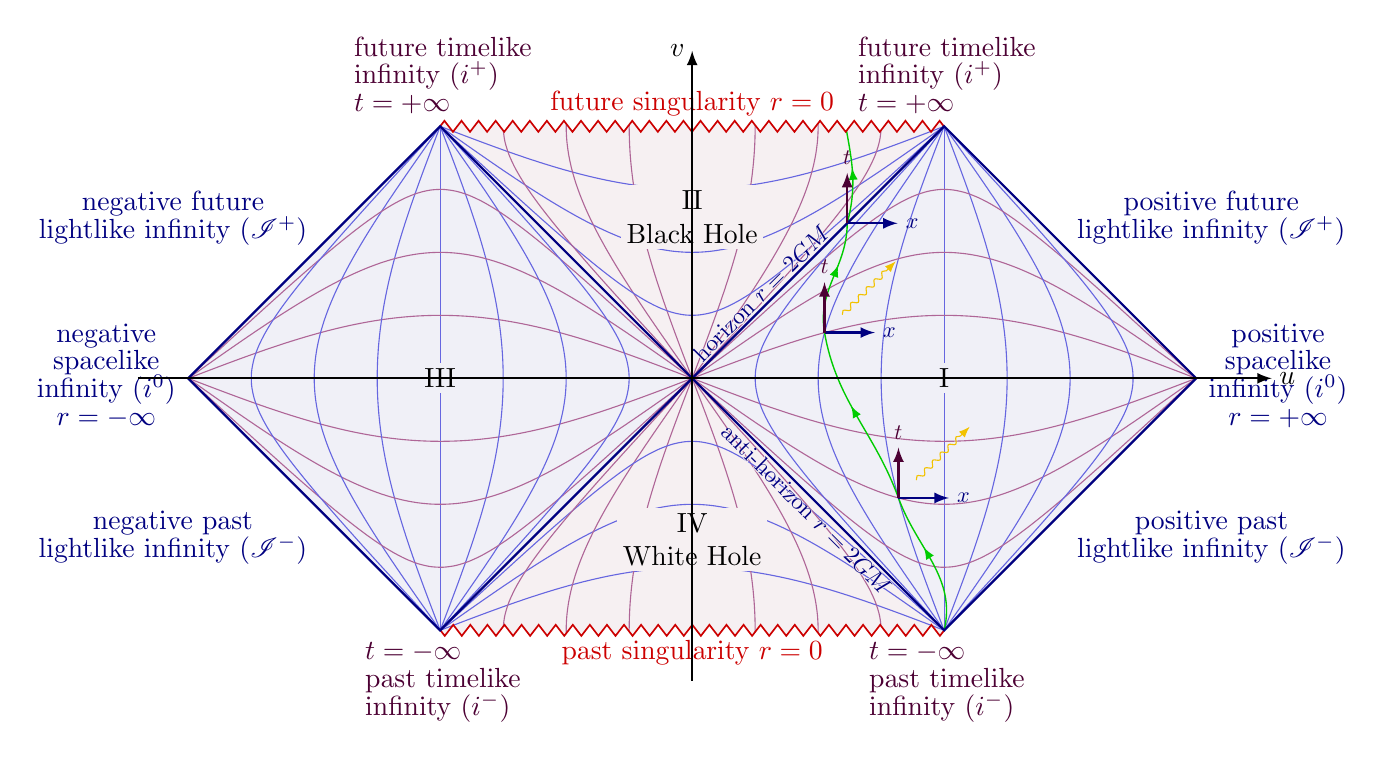
\begin{tikzpicture}[scale=3.2]
  \message{Extended Penrose diagram: Schwarzschild black hole^^J}
  
  \def\Nlines{3} % number of world lines (at constant r/t)
  \pgfmathsetmacro\ta{1/sin(90*1/(\Nlines+1))} % constant r/t value 1
  \pgfmathsetmacro\tb{sin(90*2/(\Nlines+1))}   % constant r/t value 2
  \pgfmathsetmacro\tc{1/sin(90*2/(\Nlines+1))} % constant r/t value 3
  \pgfmathsetmacro\td{sin(90*1/(\Nlines+1))}   % constant r/t value 4
  \coordinate (-O) at (-1, 0); % center III: origin (r,t) = (0,0)
  \coordinate (-S) at (-1,-1); % south III: t=-infty, i-
  \coordinate (-N) at (-1, 1); % north III: t=+infty, i+
  \coordinate (-W) at (-2, 0); % east III:  r=-infty, i0
  \coordinate (-E) at ( 0, 0); % west III:  r=+infty, i0
  \coordinate (O)  at ( 1, 0); % center I: origin (r,t) = (0,0)
  \coordinate (S)  at ( 1,-1); % south I: t=-infty, i-
  \coordinate (N)  at ( 1, 1); % north I: t=+infty, i+
  \coordinate (E)  at ( 2, 0); % east I:  r=-infty, i0
  \coordinate (W)  at ( 0, 0); % west I:  r=+infty, i0
  \coordinate (B)  at ( 0,-1); % singularity bottom
  \coordinate (T)  at ( 0, 1); % singularity top
  \coordinate (X0) at ({asin(sqrt((\ta^2-1)/(\ta^2-\tb^2)))/90},
                       {-acos(\ta*sqrt((1-\tb^2)/(\ta^2-\tb^2)))/90}); % particle 1
  \coordinate (X1) at ({asin(sqrt((\tc^2-1)/(\tc^2-\td^2)))/90},
                       {acos(\tc*sqrt((1-\td^2)/(\tc^2-\td^2)))/90}); % particle 2
  \coordinate (X2) at (45:0.87); % particle falling in BH horizon
  \coordinate (X3) at (0.60,1.05); % particle falling in BH singularity
  
  \begin{scope}
    
    % CLIP to fill inside zigzag lines
    \clip[decorate,decoration={zigzag,amplitude=2,segment length=6.17}]
      (S) -- (-S) --++ (-1.1,-0.1) |-++ (4.2,2.2) |- cycle;
    \clip[decorate,decoration={zigzag,amplitude=2,segment length=6.17}]
      (-N) -- (N) --++ (1.1,0.1) |-++ (-4.2,-2.2) |- cycle;
    
    % REGIONS FILLS
    \fill[mylightpurple] (-N) |-++ (2,0.1) -- (N) -- (-S) -- (S) -- cycle;
    \fill[mylightpurple] (-S) |-++ (2,-0.1) -- (S) -- (-N) -- (N) -- cycle;
    
    \fill[mylightblue] (-N) -- (-E) -- (-S) -- (-W) -- cycle;
    \fill[mylightblue] (N) -- (E) -- (S) -- (W) -- cycle;
    
    % WORLD LINES
    \draw[world line] (-N) -- (-S) (N) -- (S);
    \draw[world line t] (-W) -- (-E) (W) -- (E) (0,-1.1) -- (0,1.1);
    \message{Making world lines...^^J}
    \foreach \i [evaluate={\c=\i/(\Nlines+1); \cs=sin(90*\c);}] in {1,...,\Nlines}{
      \message{  Running i/N=\i/\Nlines, c=\c, cs=\cs...^^J}
      \draw[world line t,samples=2*\Nsamples,smooth,variable=\x,domain=-2:2] % region I/III, constant t
        plot(\x,{-kruskal(\x*pi/4,\cs)})
        plot(\x,{ kruskal(\x*pi/4,\cs)});
      \draw[world line,samples=\Nsamples,smooth,variable=\y,domain=0:2] % region I/III, constant r
        plot({-1-kruskal(\y*pi/4,\cs)},\y-1)
        plot({-1+kruskal(\y*pi/4,\cs)},\y-1)
        plot({1-kruskal(\y*pi/4,\cs)},\y-1)
        plot({1+kruskal(\y*pi/4,\cs)},\y-1);
      \draw[world line,samples=\Nsamples,smooth,variable=\x,domain=0:2] % region II/IV, constant r
        plot(\x-1,{kruskal(\x*pi/4,\cs)-1})
        plot(\x-1,{1-kruskal(\x*pi/4,\cs)});
      \draw[world line t,samples=\Nsamples,smooth,variable=\y,domain=-1.05:1.05] % region II/IV constant t
        plot({-kruskal(\y*pi/4,\cs)},\y)
        plot({ kruskal(\y*pi/4,\cs)},\y);
    }
    
    % PARTICLE WORLD LINE
    \draw[particle,decoration={markings,mark=at position 0.16 with {\arrow{latex}},
                                        mark=at position 0.45 with {\arrow{latex}},
                                        mark=at position 0.72 with {\arrow{latex}},
                                        mark=at position 0.90 with {\arrow{latex}}},postaction={decorate}]
      (S) to[out=77,in=-70] (X0) to[out=110,in=-80] (X1)
          to[out=100,in=-90] (X2) to[out=75,in=-80] (X3);
    
  \end{scope}
  
  % BOUNDARIES
  \draw[singularity] (-N) -- node[above] {future singularity $r=0$} (N);
  \draw[singularity] (S) -- node[below] {past singularity $r=0$} (-S);
  \path (S) -- (W) node[mydarkblue,pos=0.50,below=-2.5,rotate=-45,scale=0.85]
    {\contour{mylightpurple}{anti-horizon $r=2GM$}};
  \path (W) -- (N) node[mydarkblue,pos=0.32,above=-2.5,rotate=45,scale=0.85]
    {\contour{mylightpurple}{horizon $r=2GM$}};
  \draw[thick,mydarkblue] (-N) -- (-E) -- (-S) -- (-W) -- cycle;
  \draw[thick,mydarkblue] (N) -- (E) -- (S) -- (W) -- cycle;
  
  % REGIONS
  \node[fill=mylightblue,inner sep=2] at (-O) {III};
  \node[fill=mylightblue,inner sep=2] at (O) {I};
  \node[fill=mylightpurple,inner sep=2,align=center] at (0,0.64) {II\\Black Hole};
  \node[fill=mylightpurple,inner sep=2,align=center] at (0,-0.64) {IV\\White Hole};
  
  % SIMPLE COORDINATE ARROWS (replacing complex lightcones)
  \coordarrows{X0};
  \coordarrows{X1};
  \coordarrows{X2};
  
  % INFINITY LABELS
  \node[above=1,left=1,mydarkblue,align=center] at (-2,0) 
    {negative\\[-2]spacelike\\[-2]infinity ($i^0$)\\[-2]$r=-\infty$};
  \node[above=1,right=1,mydarkblue,align=center] at (2,0) 
    {positive\\[-2]spacelike\\[-2]infinity ($i^0$)\\[-2]$r=+\infty$};
  \node[right=1,below=1,mydarkpurple,align=left] at (-S) 
    {$t=-\infty$\\[-2]past timelike\\[-2]infinity ($i^-$)};
  \node[right=1,above=1,mydarkpurple,align=left] at (-N) 
    {future timelike\\[-2]infinity ($i^+$)\\[-2]$t=+\infty$};
  \node[right=1,below=1,mydarkpurple,align=left] at (S) 
    {$t=-\infty$\\[-2]past timelike\\[-2]infinity ($i^-$)};
  \node[right=1,above=1,mydarkpurple,align=left] at (N) 
    {future timelike\\[-2]infinity ($i^+$)\\[-2]$t=+\infty$};
  \node[mydarkblue,below left=-1,align=center] at (-1.5,-0.5) 
    {negative past\\[-2]lightlike infinity ($\calI^-$)};
  \node[mydarkblue,above left=-1,align=center] at (-1.5,0.5) 
    {negative future\\[-2]lightlike infinity ($\calI^+$)};
  \node[mydarkblue,above right=-1,align=center] at (1.5,0.5) 
    {positive future\\[-2]lightlike infinity ($\calI^+$)};
  \node[mydarkblue,below right=-1,align=center] at (1.5,-0.5) 
    {positive past\\[-2]lightlike infinity ($\calI^-$)};
  
  % ESCAPING PHOTONS
  \draw[photon] (X0) ++ (45:0.1) --++ (45:0.3);
  \draw[photon] (X1) ++ (45:0.1) --++ (45:0.3);
  
  % AXES
  \draw[->,thick] (-2.2,0) -- (2.3,0) node[right=-1] {$u$};
  \draw[->,thick] (0,-1.2) -- (0,1.3) node[left=-1] {$v$};
  
\end{tikzpicture}

% PENROSE COORDINATES for Kruskal-Szekeres coordinates
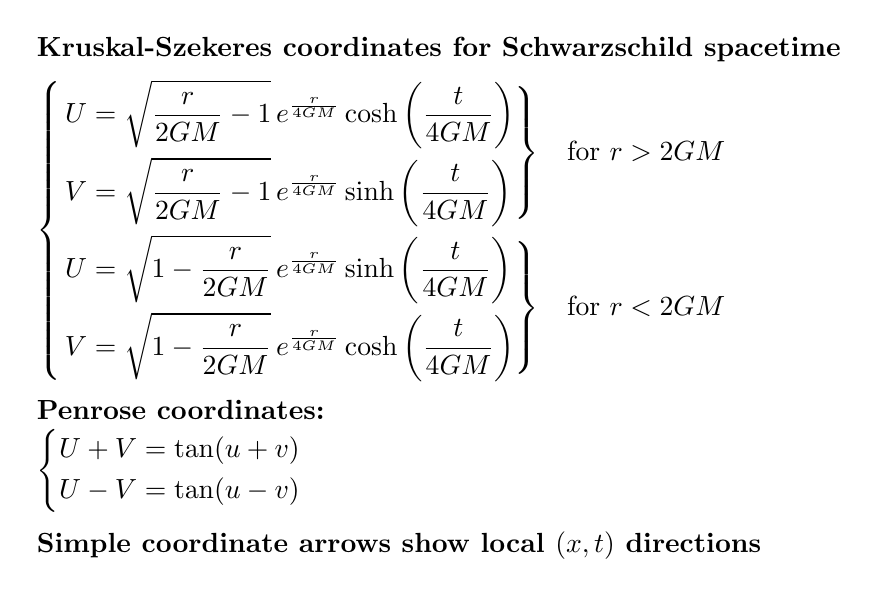
\begin{tikzpicture}[scale=1]
  \node[align=left] at (0,0) {
    \textbf{Kruskal-Szekeres coordinates for Schwarzschild spacetime}\\[2mm]
    $\displaystyle
    \begin{cases}
      \left.\begin{aligned}
        U &= \sqrt{\frac{r}{2GM}-1}\,e^{\frac{r}{4GM}}\cosh\left(\frac{t}{4GM}\right) \\
        V &= \sqrt{\frac{r}{2GM}-1}\,e^{\frac{r}{4GM}}\sinh\left(\frac{t}{4GM}\right) \\
      \end{aligned}\right\} &\text{for $r>2GM$} \\[8mm]
      \left.\begin{aligned}
        U &= \sqrt{1-\frac{r}{2GM}}\,e^{\frac{r}{4GM}}\sinh\left(\frac{t}{4GM}\right) \\
        V &= \sqrt{1-\frac{r}{2GM}}\,e^{\frac{r}{4GM}}\cosh\left(\frac{t}{4GM}\right) \\
      \end{aligned}\right\} &\text{for $r<2GM$}
    \end{cases}$\\[2mm]
    \textbf{Penrose coordinates:}\\[1mm]$
    \left\{\begin{aligned}
      U + V = \tan(u+v) \\
      U - V = \tan(u-v) \\
    \end{aligned}\right.$\\[2mm]
    \textbf{Simple coordinate arrows show local $(x,t)$ directions}
  };
\end{tikzpicture}

\end{document} 